% Options for packages loaded elsewhere
% Options for packages loaded elsewhere
\PassOptionsToPackage{unicode}{hyperref}
\PassOptionsToPackage{hyphens}{url}
\PassOptionsToPackage{dvipsnames,svgnames,x11names}{xcolor}
%
\documentclass[
  letterpaper,
  DIV=11,
  numbers=noendperiod]{scrreprt}
\usepackage{xcolor}
\usepackage{amsmath,amssymb}
\setcounter{secnumdepth}{5}
\usepackage{iftex}
\ifPDFTeX
  \usepackage[T1]{fontenc}
  \usepackage[utf8]{inputenc}
  \usepackage{textcomp} % provide euro and other symbols
\else % if luatex or xetex
  \usepackage{unicode-math} % this also loads fontspec
  \defaultfontfeatures{Scale=MatchLowercase}
  \defaultfontfeatures[\rmfamily]{Ligatures=TeX,Scale=1}
\fi
\usepackage{lmodern}
\ifPDFTeX\else
  % xetex/luatex font selection
\fi
% Use upquote if available, for straight quotes in verbatim environments
\IfFileExists{upquote.sty}{\usepackage{upquote}}{}
\IfFileExists{microtype.sty}{% use microtype if available
  \usepackage[]{microtype}
  \UseMicrotypeSet[protrusion]{basicmath} % disable protrusion for tt fonts
}{}
\makeatletter
\@ifundefined{KOMAClassName}{% if non-KOMA class
  \IfFileExists{parskip.sty}{%
    \usepackage{parskip}
  }{% else
    \setlength{\parindent}{0pt}
    \setlength{\parskip}{6pt plus 2pt minus 1pt}}
}{% if KOMA class
  \KOMAoptions{parskip=half}}
\makeatother
% Make \paragraph and \subparagraph free-standing
\makeatletter
\ifx\paragraph\undefined\else
  \let\oldparagraph\paragraph
  \renewcommand{\paragraph}{
    \@ifstar
      \xxxParagraphStar
      \xxxParagraphNoStar
  }
  \newcommand{\xxxParagraphStar}[1]{\oldparagraph*{#1}\mbox{}}
  \newcommand{\xxxParagraphNoStar}[1]{\oldparagraph{#1}\mbox{}}
\fi
\ifx\subparagraph\undefined\else
  \let\oldsubparagraph\subparagraph
  \renewcommand{\subparagraph}{
    \@ifstar
      \xxxSubParagraphStar
      \xxxSubParagraphNoStar
  }
  \newcommand{\xxxSubParagraphStar}[1]{\oldsubparagraph*{#1}\mbox{}}
  \newcommand{\xxxSubParagraphNoStar}[1]{\oldsubparagraph{#1}\mbox{}}
\fi
\makeatother

\usepackage{color}
\usepackage{fancyvrb}
\newcommand{\VerbBar}{|}
\newcommand{\VERB}{\Verb[commandchars=\\\{\}]}
\DefineVerbatimEnvironment{Highlighting}{Verbatim}{commandchars=\\\{\}}
% Add ',fontsize=\small' for more characters per line
\usepackage{framed}
\definecolor{shadecolor}{RGB}{241,243,245}
\newenvironment{Shaded}{\begin{snugshade}}{\end{snugshade}}
\newcommand{\AlertTok}[1]{\textcolor[rgb]{0.68,0.00,0.00}{#1}}
\newcommand{\AnnotationTok}[1]{\textcolor[rgb]{0.37,0.37,0.37}{#1}}
\newcommand{\AttributeTok}[1]{\textcolor[rgb]{0.40,0.45,0.13}{#1}}
\newcommand{\BaseNTok}[1]{\textcolor[rgb]{0.68,0.00,0.00}{#1}}
\newcommand{\BuiltInTok}[1]{\textcolor[rgb]{0.00,0.23,0.31}{#1}}
\newcommand{\CharTok}[1]{\textcolor[rgb]{0.13,0.47,0.30}{#1}}
\newcommand{\CommentTok}[1]{\textcolor[rgb]{0.37,0.37,0.37}{#1}}
\newcommand{\CommentVarTok}[1]{\textcolor[rgb]{0.37,0.37,0.37}{\textit{#1}}}
\newcommand{\ConstantTok}[1]{\textcolor[rgb]{0.56,0.35,0.01}{#1}}
\newcommand{\ControlFlowTok}[1]{\textcolor[rgb]{0.00,0.23,0.31}{\textbf{#1}}}
\newcommand{\DataTypeTok}[1]{\textcolor[rgb]{0.68,0.00,0.00}{#1}}
\newcommand{\DecValTok}[1]{\textcolor[rgb]{0.68,0.00,0.00}{#1}}
\newcommand{\DocumentationTok}[1]{\textcolor[rgb]{0.37,0.37,0.37}{\textit{#1}}}
\newcommand{\ErrorTok}[1]{\textcolor[rgb]{0.68,0.00,0.00}{#1}}
\newcommand{\ExtensionTok}[1]{\textcolor[rgb]{0.00,0.23,0.31}{#1}}
\newcommand{\FloatTok}[1]{\textcolor[rgb]{0.68,0.00,0.00}{#1}}
\newcommand{\FunctionTok}[1]{\textcolor[rgb]{0.28,0.35,0.67}{#1}}
\newcommand{\ImportTok}[1]{\textcolor[rgb]{0.00,0.46,0.62}{#1}}
\newcommand{\InformationTok}[1]{\textcolor[rgb]{0.37,0.37,0.37}{#1}}
\newcommand{\KeywordTok}[1]{\textcolor[rgb]{0.00,0.23,0.31}{\textbf{#1}}}
\newcommand{\NormalTok}[1]{\textcolor[rgb]{0.00,0.23,0.31}{#1}}
\newcommand{\OperatorTok}[1]{\textcolor[rgb]{0.37,0.37,0.37}{#1}}
\newcommand{\OtherTok}[1]{\textcolor[rgb]{0.00,0.23,0.31}{#1}}
\newcommand{\PreprocessorTok}[1]{\textcolor[rgb]{0.68,0.00,0.00}{#1}}
\newcommand{\RegionMarkerTok}[1]{\textcolor[rgb]{0.00,0.23,0.31}{#1}}
\newcommand{\SpecialCharTok}[1]{\textcolor[rgb]{0.37,0.37,0.37}{#1}}
\newcommand{\SpecialStringTok}[1]{\textcolor[rgb]{0.13,0.47,0.30}{#1}}
\newcommand{\StringTok}[1]{\textcolor[rgb]{0.13,0.47,0.30}{#1}}
\newcommand{\VariableTok}[1]{\textcolor[rgb]{0.07,0.07,0.07}{#1}}
\newcommand{\VerbatimStringTok}[1]{\textcolor[rgb]{0.13,0.47,0.30}{#1}}
\newcommand{\WarningTok}[1]{\textcolor[rgb]{0.37,0.37,0.37}{\textit{#1}}}

\usepackage{longtable,booktabs,array}
\newcounter{none} % for unnumbered tables
\usepackage{calc} % for calculating minipage widths
% Correct order of tables after \paragraph or \subparagraph
\usepackage{etoolbox}
\makeatletter
\patchcmd\longtable{\par}{\if@noskipsec\mbox{}\fi\par}{}{}
\makeatother
% Allow footnotes in longtable head/foot
\IfFileExists{footnotehyper.sty}{\usepackage{footnotehyper}}{\usepackage{footnote}}
\makesavenoteenv{longtable}
\usepackage{graphicx}
\makeatletter
\newsavebox\pandoc@box
\newcommand*\pandocbounded[1]{% scales image to fit in text height/width
  \sbox\pandoc@box{#1}%
  \Gscale@div\@tempa{\textheight}{\dimexpr\ht\pandoc@box+\dp\pandoc@box\relax}%
  \Gscale@div\@tempb{\linewidth}{\wd\pandoc@box}%
  \ifdim\@tempb\p@<\@tempa\p@\let\@tempa\@tempb\fi% select the smaller of both
  \ifdim\@tempa\p@<\p@\scalebox{\@tempa}{\usebox\pandoc@box}%
  \else\usebox{\pandoc@box}%
  \fi%
}
% Set default figure placement to htbp
\def\fps@figure{htbp}
\makeatother


% definitions for citeproc citations
\NewDocumentCommand\citeproctext{}{}
\NewDocumentCommand\citeproc{mm}{%
  \begingroup\def\citeproctext{#2}\cite{#1}\endgroup}
\makeatletter
 % allow citations to break across lines
 \let\@cite@ofmt\@firstofone
 % avoid brackets around text for \cite:
 \def\@biblabel#1{}
 \def\@cite#1#2{{#1\if@tempswa , #2\fi}}
\makeatother
\newlength{\cslhangindent}
\setlength{\cslhangindent}{1.5em}
\newlength{\csllabelwidth}
\setlength{\csllabelwidth}{3em}
\newenvironment{CSLReferences}[2] % #1 hanging-indent, #2 entry-spacing
 {\begin{list}{}{%
  \setlength{\itemindent}{0pt}
  \setlength{\leftmargin}{0pt}
  \setlength{\parsep}{0pt}
  % turn on hanging indent if param 1 is 1
  \ifodd #1
   \setlength{\leftmargin}{\cslhangindent}
   \setlength{\itemindent}{-1\cslhangindent}
  \fi
  % set entry spacing
  \setlength{\itemsep}{#2\baselineskip}}}
 {\end{list}}
\usepackage{calc}
\newcommand{\CSLBlock}[1]{\hfill\break\parbox[t]{\linewidth}{\strut\ignorespaces#1\strut}}
\newcommand{\CSLLeftMargin}[1]{\parbox[t]{\csllabelwidth}{\strut#1\strut}}
\newcommand{\CSLRightInline}[1]{\parbox[t]{\linewidth - \csllabelwidth}{\strut#1\strut}}
\newcommand{\CSLIndent}[1]{\hspace{\cslhangindent}#1}



\setlength{\emergencystretch}{3em} % prevent overfull lines

\providecommand{\tightlist}{%
  \setlength{\itemsep}{0pt}\setlength{\parskip}{0pt}}



 


\KOMAoption{captions}{tableheading}
\makeatletter
\@ifpackageloaded{tcolorbox}{}{\usepackage[skins,breakable]{tcolorbox}}
\@ifpackageloaded{fontawesome5}{}{\usepackage{fontawesome5}}
\definecolor{quarto-callout-color}{HTML}{909090}
\definecolor{quarto-callout-note-color}{HTML}{0758E5}
\definecolor{quarto-callout-important-color}{HTML}{CC1914}
\definecolor{quarto-callout-warning-color}{HTML}{EB9113}
\definecolor{quarto-callout-tip-color}{HTML}{00A047}
\definecolor{quarto-callout-caution-color}{HTML}{FC5300}
\definecolor{quarto-callout-color-frame}{HTML}{acacac}
\definecolor{quarto-callout-note-color-frame}{HTML}{4582ec}
\definecolor{quarto-callout-important-color-frame}{HTML}{d9534f}
\definecolor{quarto-callout-warning-color-frame}{HTML}{f0ad4e}
\definecolor{quarto-callout-tip-color-frame}{HTML}{02b875}
\definecolor{quarto-callout-caution-color-frame}{HTML}{fd7e14}
\makeatother
\makeatletter
\@ifpackageloaded{bookmark}{}{\usepackage{bookmark}}
\makeatother
\makeatletter
\@ifpackageloaded{caption}{}{\usepackage{caption}}
\AtBeginDocument{%
\ifdefined\contentsname
  \renewcommand*\contentsname{Table of contents}
\else
  \newcommand\contentsname{Table of contents}
\fi
\ifdefined\listfigurename
  \renewcommand*\listfigurename{List of Figures}
\else
  \newcommand\listfigurename{List of Figures}
\fi
\ifdefined\listtablename
  \renewcommand*\listtablename{List of Tables}
\else
  \newcommand\listtablename{List of Tables}
\fi
\ifdefined\figurename
  \renewcommand*\figurename{Figure}
\else
  \newcommand\figurename{Figure}
\fi
\ifdefined\tablename
  \renewcommand*\tablename{Table}
\else
  \newcommand\tablename{Table}
\fi
}
\@ifpackageloaded{float}{}{\usepackage{float}}
\floatstyle{ruled}
\@ifundefined{c@chapter}{\newfloat{codelisting}{h}{lop}}{\newfloat{codelisting}{h}{lop}[chapter]}
\floatname{codelisting}{Listing}
\newcommand*\listoflistings{\listof{codelisting}{List of Listings}}
\makeatother
\makeatletter
\makeatother
\makeatletter
\@ifpackageloaded{caption}{}{\usepackage{caption}}
\@ifpackageloaded{subcaption}{}{\usepackage{subcaption}}
\makeatother
\usepackage{bookmark}
\IfFileExists{xurl.sty}{\usepackage{xurl}}{} % add URL line breaks if available
\urlstyle{same}
\hypersetup{
  pdftitle={Stats 141. Introduction to Statistics for Biology},
  colorlinks=true,
  linkcolor={blue},
  filecolor={Maroon},
  citecolor={Blue},
  urlcolor={Blue},
  pdfcreator={LaTeX via pandoc}}


\title{Stats 141. Introduction to Statistics for Biology}
\author{}
\date{}
\begin{document}
\maketitle

\renewcommand*\contentsname{Table of contents}
{
\setcounter{tocdepth}{2}
\tableofcontents
}

\bookmarksetup{startatroot}

\chapter*{Syllabus}\label{syllabus}
\addcontentsline{toc}{chapter}{Syllabus}

\markboth{Syllabus}{Syllabus}

\textbf{Spring 2026}

Lectures: MWF, 9:30-10:50, CODA B90.

Discussion section: Th (times below)

\textbf{Course staff, office hours, and section times:}

{\def\LTcaptype{none} % do not increment counter
\begin{longtable}[]{@{}
  >{\raggedright\arraybackslash}p{(\linewidth - 6\tabcolsep) * \real{0.2432}}
  >{\raggedright\arraybackslash}p{(\linewidth - 6\tabcolsep) * \real{0.2432}}
  >{\raggedright\arraybackslash}p{(\linewidth - 6\tabcolsep) * \real{0.2432}}
  >{\raggedright\arraybackslash}p{(\linewidth - 6\tabcolsep) * \real{0.2703}}@{}}
\toprule\noalign{}
\begin{minipage}[b]{\linewidth}\raggedright
Name
\end{minipage} & \begin{minipage}[b]{\linewidth}\raggedright
Role
\end{minipage} & \begin{minipage}[b]{\linewidth}\raggedright
Office hours
\end{minipage} & \begin{minipage}[b]{\linewidth}\raggedright
Discussion section
\end{minipage} \\
\midrule\noalign{}
\endhead
\bottomrule\noalign{}
\endlastfoot
Julia Palacios & Instructor & W 11:00-12:00 in CoDa E250 & \\
Aditya Ghosh & TA & TBC & Th 9:30-10:20am in Lathrop 015, 2:30-3:20pm in
Thronton 211 \\
Jing Shang & TA & TBC & Th 9:30-10:20am in 160-127, 2:30-3:20pm in
Thronton 210 \\
\end{longtable}
}

\section*{Contact}\label{contact}
\addcontentsline{toc}{section}{Contact}

\markright{Contact}

If you need to reach us outside of lectures, tutorials or office hours,
please contact us on the
\href{https://edstem.org/us/courses/96989/discussion}{Ed Discussion
forum}.

\section*{Overview}\label{overview}
\addcontentsline{toc}{section}{Overview}

\markright{Overview}

This is an introductory course in statistics for students specializing
in the life sciences. The emphasis is on statistical ideas rather than
computations or mathematical formulations. There are no prerequisites
except elementary algebra.

In this course, students will:

\begin{enumerate}
\def\labelenumi{(\arabic{enumi})}
\item
  Learn to identify key statistical issues to be addressed during the
  design phase of an experiment (e.g., threats to conclusion,
  identifying confounders, appropriate measurements, randomization).
\item
  Become proficient with intermediate statistical methods: comparing
  groups (analysis of variance); analyzing associations (linear
  regression); and methods for categorical data (contingency tables and
  odds ratio). You should know which methods are useful in different
  situations, and which conditions have to be checked for the method to
  be applicable.
\item
  Be able to perform detailed data analyses on a variety of biological
  data using the statistical computation environment R, including basic
  programming. You should be able to implement all the methods discussed
  in this course.
\end{enumerate}

\subsection*{Materials, Tools, \&
Resources}\label{materials-tools-resources}
\addcontentsline{toc}{subsection}{Materials, Tools, \& Resources}

\begin{enumerate}
\def\labelenumi{(\arabic{enumi})}
\item
  \textbf{Course website}. This is the course website. Here you will
  find the course schedule, lecture slides, assignments, and practice
  quizzes.
\item
  \textbf{Lecture slides}. Lecture slides are the primary source of
  information for the course; they will be made available online after
  lecture.
\item
  \textbf{Textbooks}. There is no required textbook, however material is
  based on the following:
\end{enumerate}

\begin{itemize}
\tightlist
\item
  Statistics for the Life Sciences, 5th Edition by Samules, Witmer, and
  Schaffner.
\item
  The Analysis of Biological Data, 3rd Edition by Whitlock, Schluter.
\end{itemize}

\begin{enumerate}
\def\labelenumi{(\arabic{enumi})}
\setcounter{enumi}{3}
\item
  \textbf{Gradescope}. Feedback on your quizzes and the final exam will
  be available on
  \href{https://canvas.stanford.edu/courses/224513/external_tools/74302}{gradescope}.
\item
  \textbf{Ed}. We will use Ed as an online class forum, where you may
  ask questions and discuss with your fellow students. Students are
  encouraged to answer each others' questions, and participation points
  will be awarded accordingly. The TAs will periodically review Ed to
  provide clarification, as needed, and to endorse student answers. You
  can access the Ed forum for the class
  \href{https://edstem.org/us/courses/96989/discussion}{here} or through
  Canvas.
\item
  \textbf{R resources}. In this course, computation will be done in R.
  We recommend the free versions of the following software:

  *\href{https://cloud.r-project.org/}{R}

  *\href{https://posit.co/download/rstudio-desktop/}{RStudio}

  *\href{https://r4ds.hadley.nz/}{Great tutorial}
\end{enumerate}

If you have any installation difficulties or questions please ask your
TAs

\begin{enumerate}
\def\labelenumi{(\arabic{enumi})}
\setcounter{enumi}{6}
\tightlist
\item
  \textbf{AI}. The course policy of STATS 141 is to embrace AI.
\end{enumerate}

\begin{itemize}
\item
  Some section assignments will be need some programming. Whether or not
  you know how to program, you can use AI to complete programming
  assignments. We will provide you with guidance and suggestions.
\item
  If you would like, you may also use AI to help you study for the
  course. Beware that AI agents are still susceptible to mistakes, and
  that you are ultimately fully responsible for your own understanding.
\end{itemize}

\begin{enumerate}
\def\labelenumi{(\arabic{enumi})}
\setcounter{enumi}{7}
\tightlist
\item
  \textbf{Accommodations.} Students who may need an academic
  accommodation based on the impact of a disability must initiate the
  request with the Office of Accessible Education (OAE). If you plan to
  use your OAE-approved exam accommodations for a specific assessment,
  you must provide your letter and inform the instructor 10 days before
  the exam.
\end{enumerate}

\section*{Coursework \& Evaluation}\label{coursework-evaluation}
\addcontentsline{toc}{section}{Coursework \& Evaluation}

\markright{Coursework \& Evaluation}

\begin{enumerate}
\def\labelenumi{(\arabic{enumi})}
\tightlist
\item
  \textbf{Quizzes (45\%)}
\end{enumerate}

\begin{itemize}
\tightlist
\item
  We will have a quiz in class every Friday.
\item
  Your two lowest quiz scores will be dropped.
\end{itemize}

\begin{enumerate}
\def\labelenumi{(\arabic{enumi})}
\setcounter{enumi}{1}
\tightlist
\item
  \textbf{Final Exam (45\%)}
\end{enumerate}

\begin{itemize}
\tightlist
\item
  The final will be in-person during finals week on Tuesday, June 9,
  2026 at 8:30am
\item
  Students must be present for the final.
\item
  If your final grade is higher than your average quiz grade (after
  dropping the lowest two), we will replace your quiz grade with your
  final grade.
\end{itemize}

\begin{enumerate}
\def\labelenumi{(\arabic{enumi})}
\setcounter{enumi}{2}
\tightlist
\item
  \textbf{Section participation and Lecture worksheets (10\%)}
\end{enumerate}

\begin{itemize}
\tightlist
\item
  Each week, you will be given a hands-on assignment to complete ahead
  of section.
\item
  In section you will turn in your assignment, and discuss and share
  your results with classmates.
\item
  There will be a worksheet for students to fill out accompanying each
  lecture.
\end{itemize}

\section*{Units}\label{units}
\addcontentsline{toc}{section}{Units}

\markright{Units}

\begin{enumerate}
\def\labelenumi{(\arabic{enumi})}
\tightlist
\item
  Introduction to Statistics and EDA
\item
  Generative Models for Discrete and Continuous Data
\item
  Sampling Distributions
\item
  Inference for Means
\item
  Statistical Models
\item
  Design of experiments
\end{enumerate}

\section*{Regrade Policy}\label{regrade-policy}
\addcontentsline{toc}{section}{Regrade Policy}

\markright{Regrade Policy}

If you believe that we have made a mistake in grading, please e-mail
Prof.~Palacios within 1 week of getting the assignment/exam back. Note
that Professor Palacios will regrade your entire assignment/exam, so
your grade could go up or down.

\section*{The Honor Code}\label{the-honor-code}
\addcontentsline{toc}{section}{The Honor Code}

\markright{The Honor Code}

It is expected that instructors and students will follow Stanford's
Honor Code in all matters relating to this course. You are encouraged to
meet and exchange ideas with your classmates while studying and working
on homework assignments, but you are individually responsible for your
own work and for understanding the material. You are not permitted to
copy or otherwise reference another student's homework or computer code.
If you have any questions regarding this policy, feel free to contact
me.

Compromising your academic integrity may lead to serious consequences,
including (but not limited to) one or more of the following: failure of
the assignment, failure of the course, disciplinary probation,
suspension from the university, or dismissal from the university.

Students are responsible for understanding the University's Honor Code
policy and must make proper use of citations of sources for writing
papers, creating, presenting, and performing their work, taking
examinations, and doing research.

\section*{Course Privacy Statement}\label{course-privacy-statement}
\addcontentsline{toc}{section}{Course Privacy Statement}

\markright{Course Privacy Statement}

As noted in the University's
\href{https://library.stanford.edu/using/copyright-reminder/common-situations/recording-broadcasting-courses}{policy on recording and broadcasting courses},
students may not audio or video record class meetings without permission
from the instructor (and guest speakers, when applicable).

\part{Activities}

\part{Activities}

\textbf{Need for control groups}. An experiment was conducted in which
subjects were given the drug clofibrate, which was intended to lower
cholesterol and reduce the chance of death from coronary disease. The
researchers noted that many of the subjects did not take all the
medication that the experimental protocol called for them to take. They
calculated the percentage of the prescribed capsules that each subject
took and divided the subjects into two groups according to whether or
not the subjects took at least \(80%
\) of the capsules they were given. The next table shows that the
five-year mortality rate for those who took at least \(80%
\) of their capsules was much lower than the corresponding rate for
subjects who did not adhere to the protocol. On the surface, this
suggests that taking the medication lowers the chance of death. However,
there was a placebo control group in the experiment and many of the
placebo subjects took fewer than \(80%
\) of their capsules. The mortality rates for the two placebo
groups---those who adhered to the protocol and those who did not---are
quite similar to the rates for the clofibrate groups.

\begin{enumerate}
\def\labelenumi{(\arabic{enumi})}
\tightlist
\item
  What can you conclude?
\item
  What could explain the differences between the two rows?
\item
  What would have happened in the absence of the placebo control group?
\end{enumerate}

\chapter{Summary}\label{summary}

In summary, this book has no content whatsoever.

\begin{Shaded}
\begin{Highlighting}[]
\DecValTok{1} \SpecialCharTok{+} \DecValTok{1}
\end{Highlighting}
\end{Shaded}

\begin{verbatim}
[1] 2
\end{verbatim}

\bookmarksetup{startatroot}

\chapter{Introduction to Statistics}\label{introduction-to-statistics}

\textbf{Statistics}

Researchers in the life sciences analyze \textbf{data} that exhibit some
\textbf{variability}. For example, patients given the same treatment may
respond differently; PCR (Polymerase Chain Reaction) prepared
identically may have different results due to contamination, thermal
damage, etc. The challenge to the life scientist is to discern the
\textbf{signal} from the \textbf{noise}.

\textbf{Statistics} is the science of understanding data (collection,
analysis and presentation) and of making decisions in the face of
variability and uncertainty. Statistics is a core component of
\textbf{data science}.

\begin{figure}[H]

{\centering 
\includegraphics[width=0.5\linewidth,height=\textheight,keepaspectratio]{Figures/DataScience.ppm}

}

\caption{Data Science, credit: Lee et al.~2018}

\end{figure}%

\textbf{Experimental Design}

Researchers gather information to make inferences about nature in a
variety of settings. Much of statistics deals with \textbf{data
analysis}, but statistical considerations often play a key role in the
planning and design of scientific investigation.

\begin{tcolorbox}[enhanced jigsaw, arc=.35mm, bottomrule=.15mm, bottomtitle=1mm, breakable, colback=white, colbacktitle=quarto-callout-note-color!10!white, colframe=quarto-callout-note-color-frame, coltitle=black, left=2mm, leftrule=.75mm, opacityback=0, opacitybacktitle=0.6, rightrule=.15mm, title={Example: Health and Marriage}, titlerule=0mm, toprule=.15mm, toptitle=1mm]

A study conducted in Finland found that people who were married at
midlife were less likely to develop cognitive impairment (particularly
Alzheimer's disease) later in life. However, from an
\textbf{observational} study such as this we don't know whether marriage
prevents later problems or whether persons who are likely to develop
cognitive problems are less likely to get married.

\end{tcolorbox}

\begin{tcolorbox}[enhanced jigsaw, arc=.35mm, bottomrule=.15mm, bottomtitle=1mm, breakable, colback=white, colbacktitle=quarto-callout-note-color!10!white, colframe=quarto-callout-note-color-frame, coltitle=black, left=2mm, leftrule=.75mm, opacityback=0, opacitybacktitle=0.6, rightrule=.15mm, title={Example: Sexual orientation}, titlerule=0mm, toprule=.15mm, toptitle=1mm]

Some research has suggested that there is a genetic basis for sexual
orientation. One such study involved measuring the midsagittal area of
he anterior commissure (AC) of the brain for 30 homosexual men, 30
heterosexual men, and 30 heterosexual women. The research found that the
AC tends to be larger in heterosexual women than in heterosexual men and
that it is even larger in homosexual men.

\end{tcolorbox}

\begin{figure}[H]

{\centering 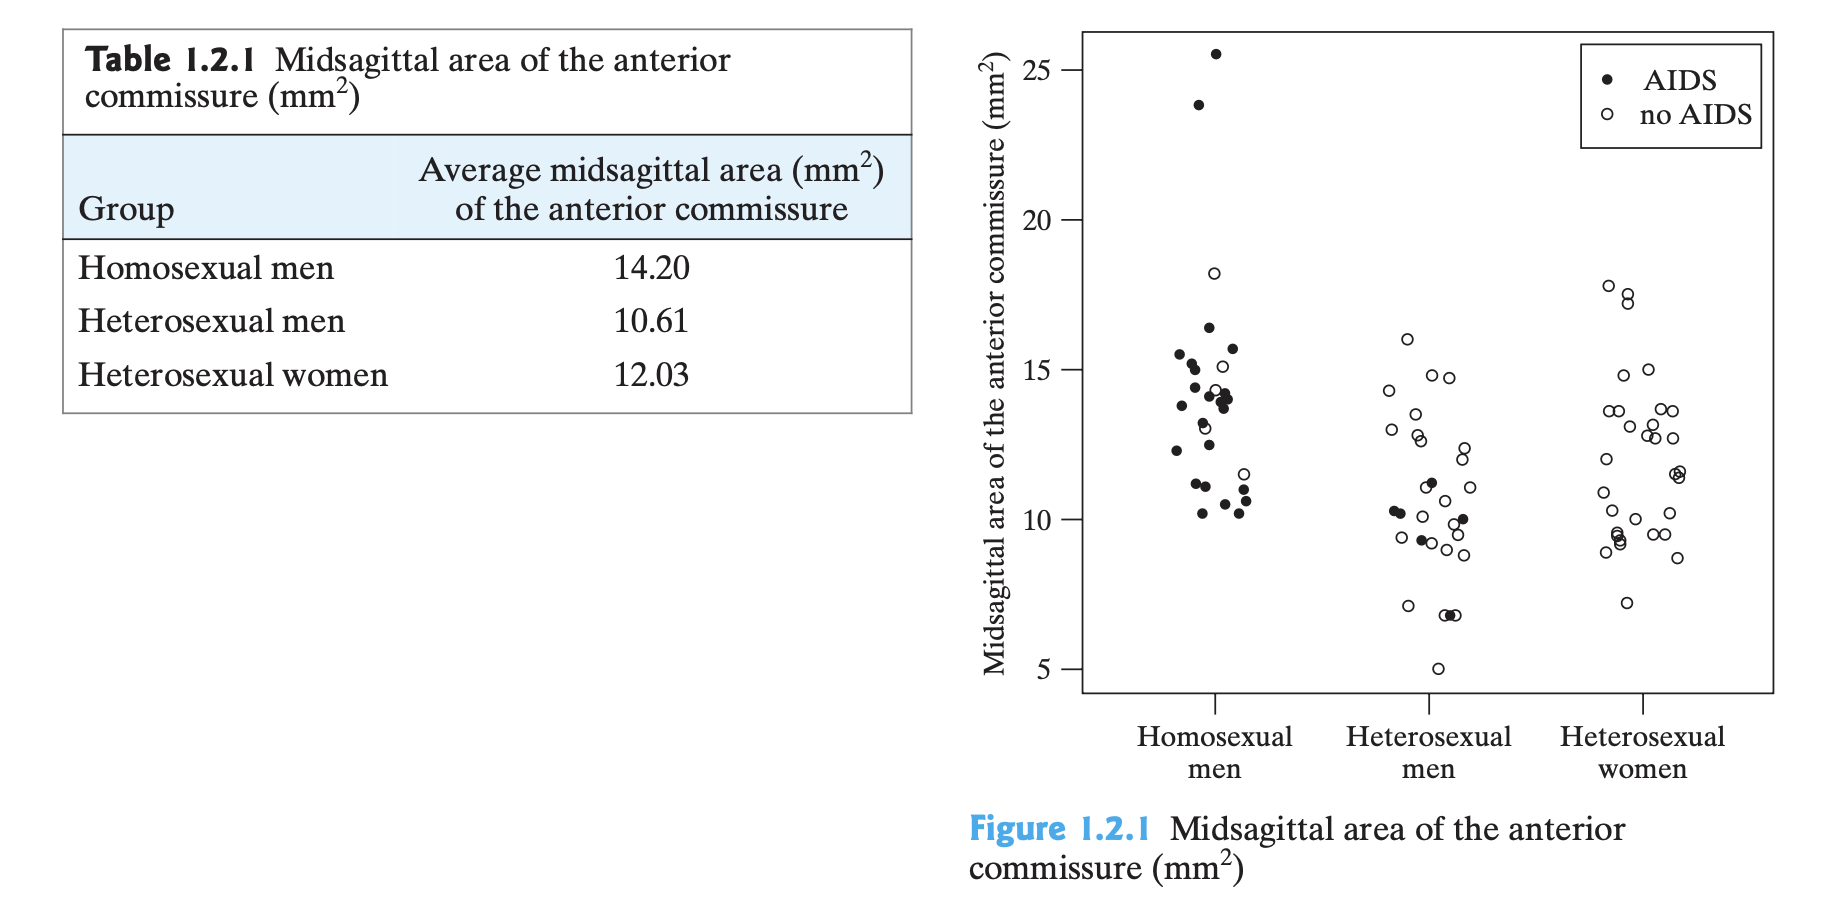
\includegraphics[width=0.95\linewidth,height=\textheight,keepaspectratio]{Figures/Samuels1.png}

}

\caption{credit: SWS Book}

\end{figure}%

The previous two examples are based on \textbf{observational studies}.
In an observational study the researcher systematically collects data
from subjects, but only as an observer and not as someone who is
manipulating the conditions. However, observational studies can be
misleading due to \textbf{confounding variables}. The context in which
the data arose is important and tell us to be on the alert for the
effects that other factors, such as the impact of AIDS, may have on the
size of the anterior commissure.

\textbf{Confounders} are variables, other than the treatment, which are
responsible for causing (at least part of) the observed difference in
the outcome between the various levels of the treatment.

\textbf{How can we mitigate confounding?} Create treatment and control
groups that are as similar as possible except for the treatment level
and we can anticipate and prevent both other known and unknown
explanations for the observed difference in outcomes between the treated
and control groups.

\begin{tcolorbox}[enhanced jigsaw, arc=.35mm, bottomrule=.15mm, bottomtitle=1mm, breakable, colback=white, colbacktitle=quarto-callout-note-color!10!white, colframe=quarto-callout-note-color-frame, coltitle=black, left=2mm, leftrule=.75mm, opacityback=0, opacitybacktitle=0.6, rightrule=.15mm, title={Example: Toxicity in Dogs}, titlerule=0mm, toprule=.15mm, toptitle=1mm]

In part of one study, a new investigational drug was given to eight male
and eight female dogs at doses of \(8 mg/kg\) and \(25 mg/kg\). Within
each sex, the two doses were assigned at random to the eight dogs. Many
``endpoints'' were measured, such as cholesterol, sodium, glucose, and
so on, from blood samples, in order to screen for toxicity problems in
the dogs before starting studies on humans. One endpoint was alkaline
phosphatase level (or APL, measured in \(U/l\)).

\end{tcolorbox}

\begin{figure}[H]

{\centering 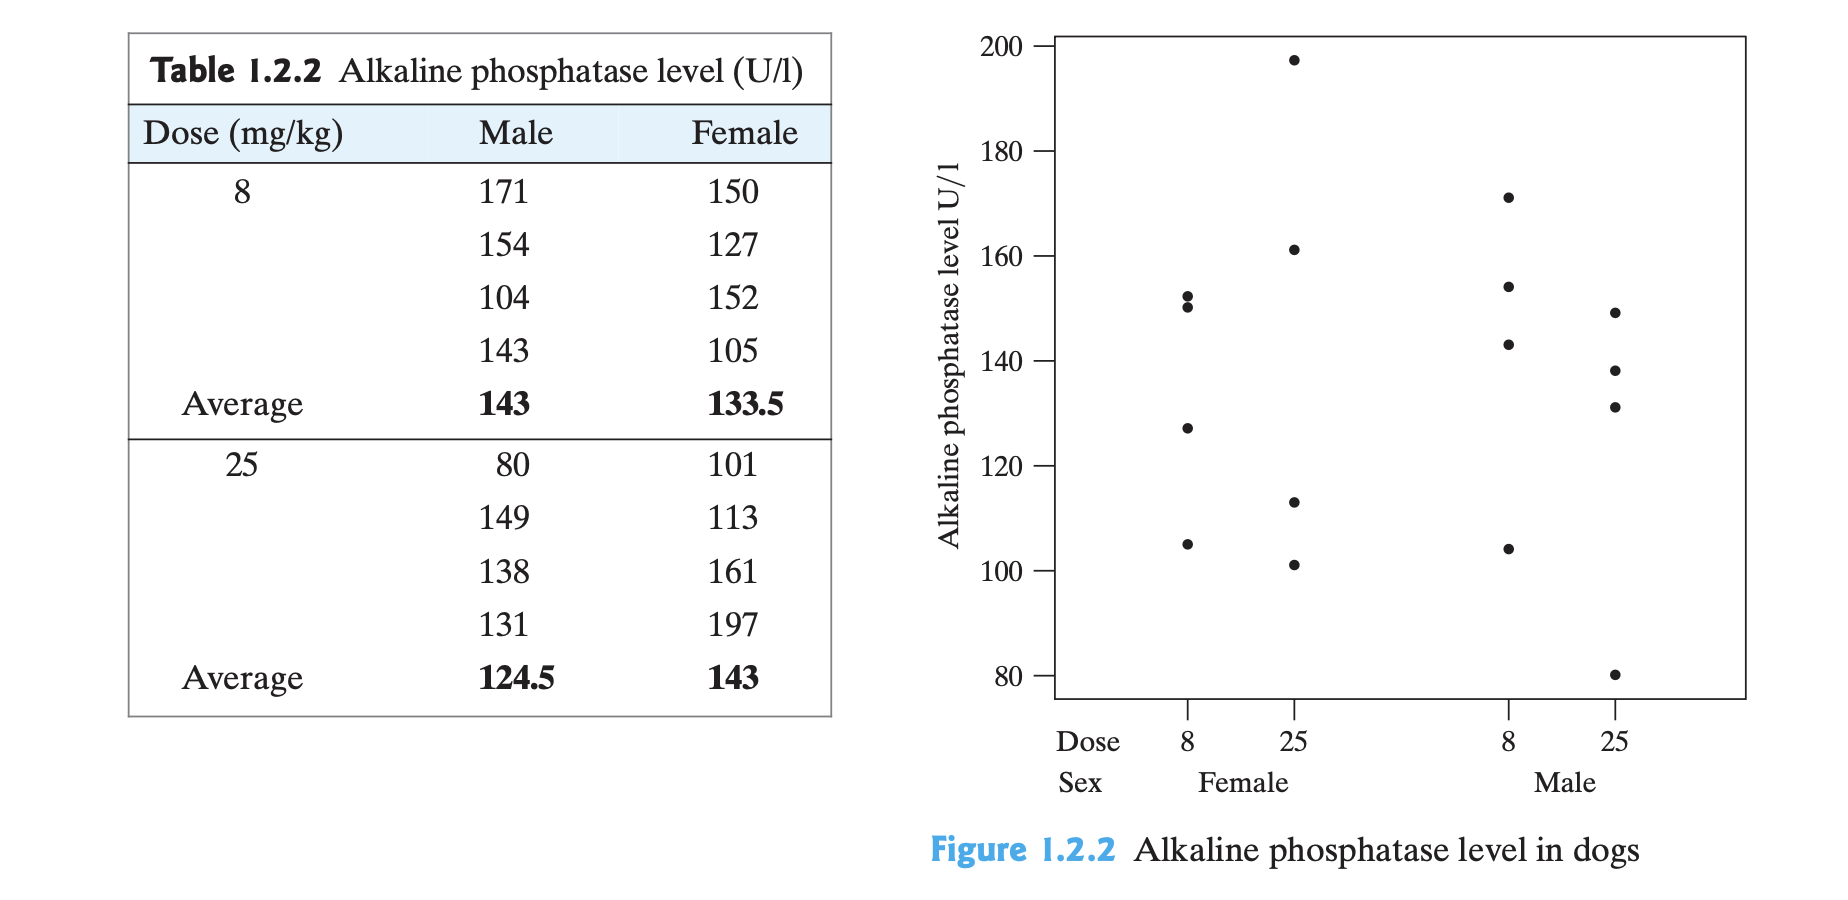
\includegraphics[width=0.95\linewidth,height=\textheight,keepaspectratio]{Figures/Samuels2.png}

}

\caption{credit: SWS Book}

\end{figure}%

The \textbf{design of this experiment} allows for the investigation of
the \textbf{interaction} between two factors: sex of the dog and dose.
That is, for females, the effect of increasing the dose from 8 to 25
mg/kg was positive, although small (from 133.5 to 143 \(U/l\)), but for
males the effect of increasing the dose from 8 to 25 \(mg/kg\) was
negative (from 143 to 124.5 \(U/l\)).

By \textbf{randomly assigning} treatments (drug doses) to subjects
(dogs), we can get around the problem of confounding that complicates
observational studies and limits the conclusions. \textbf{Randomized
experiments} are considered the gold standard in scientific
investigation, but they can also be difficult.

Often, human subjects in experiments are given a \textbf{placebo}. Of
course, if a placebo control is used, then the subjects must not be told
which group they are in, that is, the experiment is \textbf{blinded}.
The purpose of blinding is to minimize the extent to which subject
expectations influence the results of the experiment. If subjects
exhibit a psychological reaction to getting a medication, that placebo
response will tend to balance out between the two groups, so that any
difference between the groups can be attributed to the effect of the
active treatment.

\begin{figure}[H]

{\centering 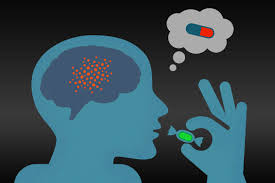
\includegraphics[width=0.5\linewidth,height=\textheight,keepaspectratio]{Figures/placebo.jpeg}

}

\caption{credit: Javier Zarracina - Vox}

\end{figure}%

How about the person evaluating the responses? This person can be
subject to bias influencing the observation process itself. An
experiment in which both the subjects and the persons making the
evaluations of the response are blinded is called
\textbf{double-blinded}.

\%\%Activity on the need for control groups

\textbf{Exploratory Data Analysis (EDA)}

\textbf{Confirmatory Data Analysis (CDA)}

See Knuth (1984) for additional discussion of literate programming.

\begin{Shaded}
\begin{Highlighting}[]
\DecValTok{1} \SpecialCharTok{+} \DecValTok{1}
\end{Highlighting}
\end{Shaded}

\begin{verbatim}
[1] 2
\end{verbatim}

\bookmarksetup{startatroot}

\chapter{Summary}\label{summary-1}

In summary, this book has no content whatsoever.

\begin{Shaded}
\begin{Highlighting}[]
\DecValTok{1} \SpecialCharTok{+} \DecValTok{1}
\end{Highlighting}
\end{Shaded}

\begin{verbatim}
[1] 2
\end{verbatim}

\bookmarksetup{startatroot}

\chapter*{References}\label{references}
\addcontentsline{toc}{chapter}{References}

\markboth{References}{References}

\protect\phantomsection\label{refs}
\begin{CSLReferences}{1}{1}
\bibitem[\citeproctext]{ref-knuth84}
Knuth, Donald E. 1984. {``Literate Programming.''} \emph{Comput. J.}
(USA) 27 (2): 97--111. \url{https://doi.org/10.1093/comjnl/27.2.97}.

\end{CSLReferences}

\part{Discussion.qmd}

\chapter{Summary}\label{summary-2}

In summary, this book has no content whatsoever.

\begin{Shaded}
\begin{Highlighting}[]
\DecValTok{1} \SpecialCharTok{+} \DecValTok{1}
\end{Highlighting}
\end{Shaded}

\begin{verbatim}
[1] 2
\end{verbatim}

\chapter{Summary}\label{summary-3}

In summary, this book has no content whatsoever.

\begin{Shaded}
\begin{Highlighting}[]
\DecValTok{1} \SpecialCharTok{+} \DecValTok{1}
\end{Highlighting}
\end{Shaded}

\begin{verbatim}
[1] 2
\end{verbatim}




\end{document}
